%!TEX root = ../thesis.tex
%*******************************************************************************
%****************************** Fourth Chapter *********************************
%*******************************************************************************

\chapter{Resultados}

\ifpdf
    \graphicspath{{Chapter4/Figs/}{Chapter4/Figs/PDF/}{Chapter4/Figs/}}
\else
    \graphicspath{{Chapter4/Figs/}{Chapter4/Figs/}}
\fi


\section{Resultados}

\subsection{Aplicación}
La aplicación resultante es una plataforma de crowdfunding donde los usuarios que aporten 
a los proyectos, además deberán aprobar solicitudes de pagos creadas por el owner del proyecto.
Sin éstas, el dinero del proyecto no podrá ser movido de la plataforma.

La aplicación consta de, por un lado, el frontend programado en React quien por medio de la 
librería web3 se puede conectar directamente con el contrato deployado y usar sus métodos a modo
de API. El contrato en sí mismo actúa como base de datos en Ethereum.

Por otro lado, en la aplicación encontramos el contrato escrito en Solidity, todos los scripts
relacionados a él (compilar, deployar, obtener proyecto y obtener la factory), y los tests
correspondientes a estos scripts.

A continuación pondré una serie de screenshots de la aplicación en donde se verán las distintas
secciones y páginas que componen la misma acompañadas de breves descripciones en el pie de foto.

\begin{figure}[H] 
\centering    
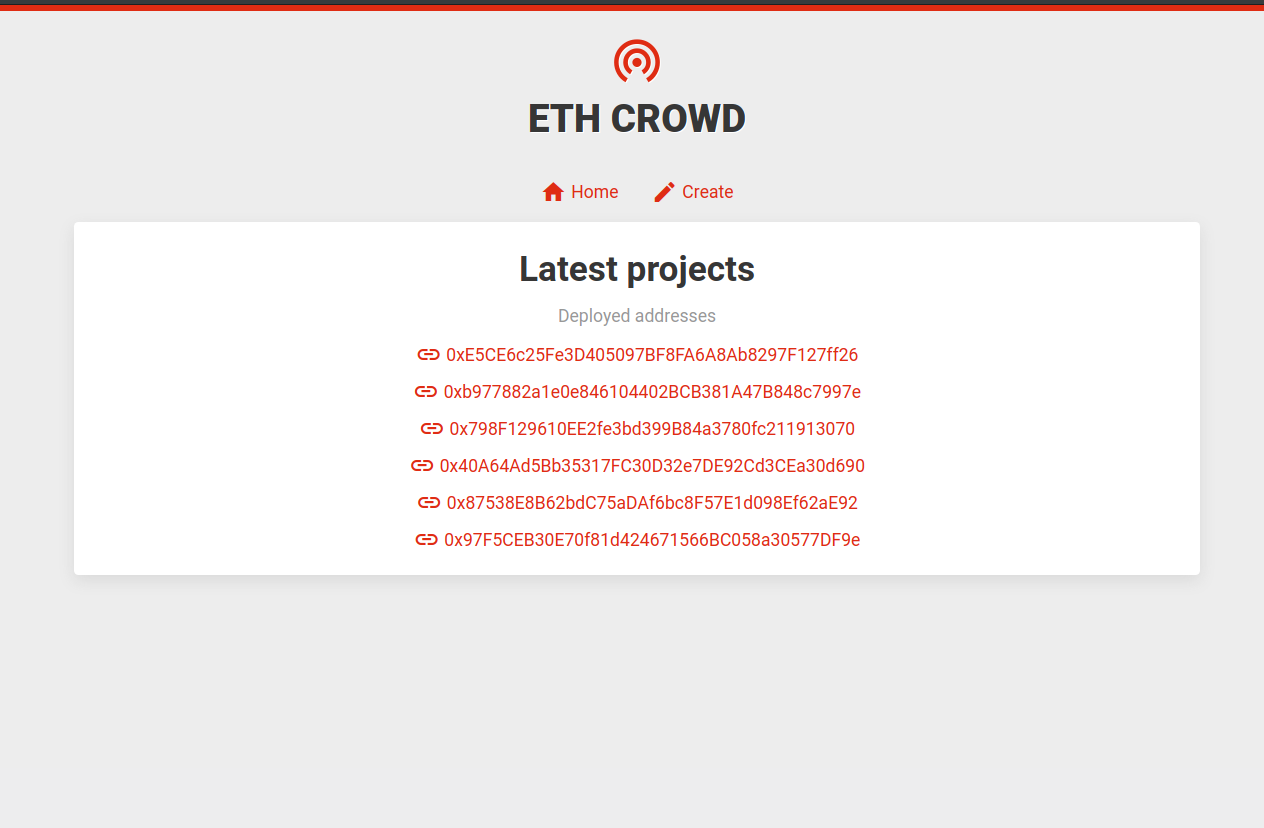
\includegraphics[width=0.9\textwidth]{home}
\caption[home]{En la home se pueden ver todas las direcciones de los proyectos deployados en el contrato Ethereum.}
\label{fig:home}
\end{figure}

\begin{figure}[H] 
\centering    
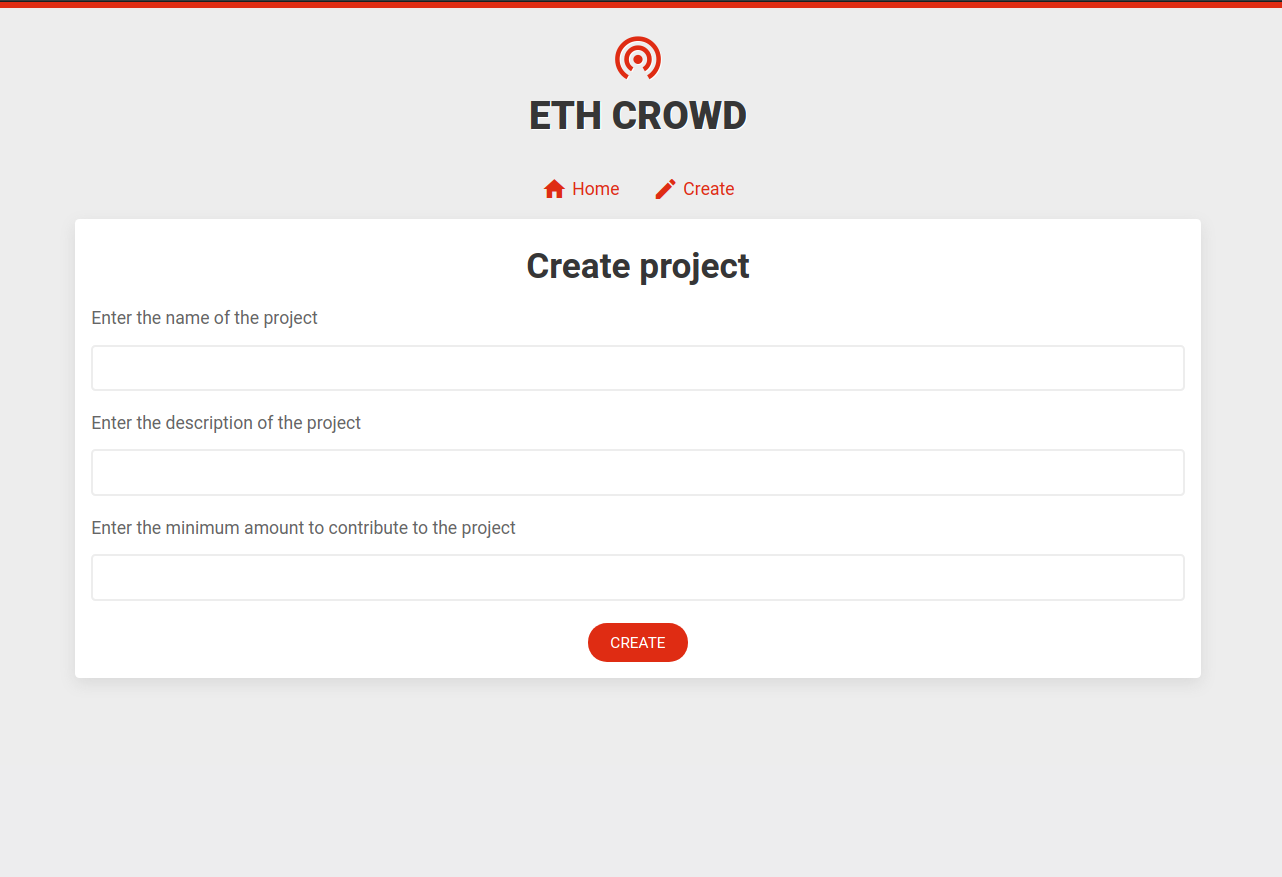
\includegraphics[width=0.9\textwidth]{new-project}
\caption[new-project]{El formulario que se muestra aquí es el utilizado para crear nuevos proyectos. Los tres inputs que se presentan son requeridos para el proceso de creación.}
\label{fig:new-project}
\end{figure}

\begin{figure}[H] 
\centering    
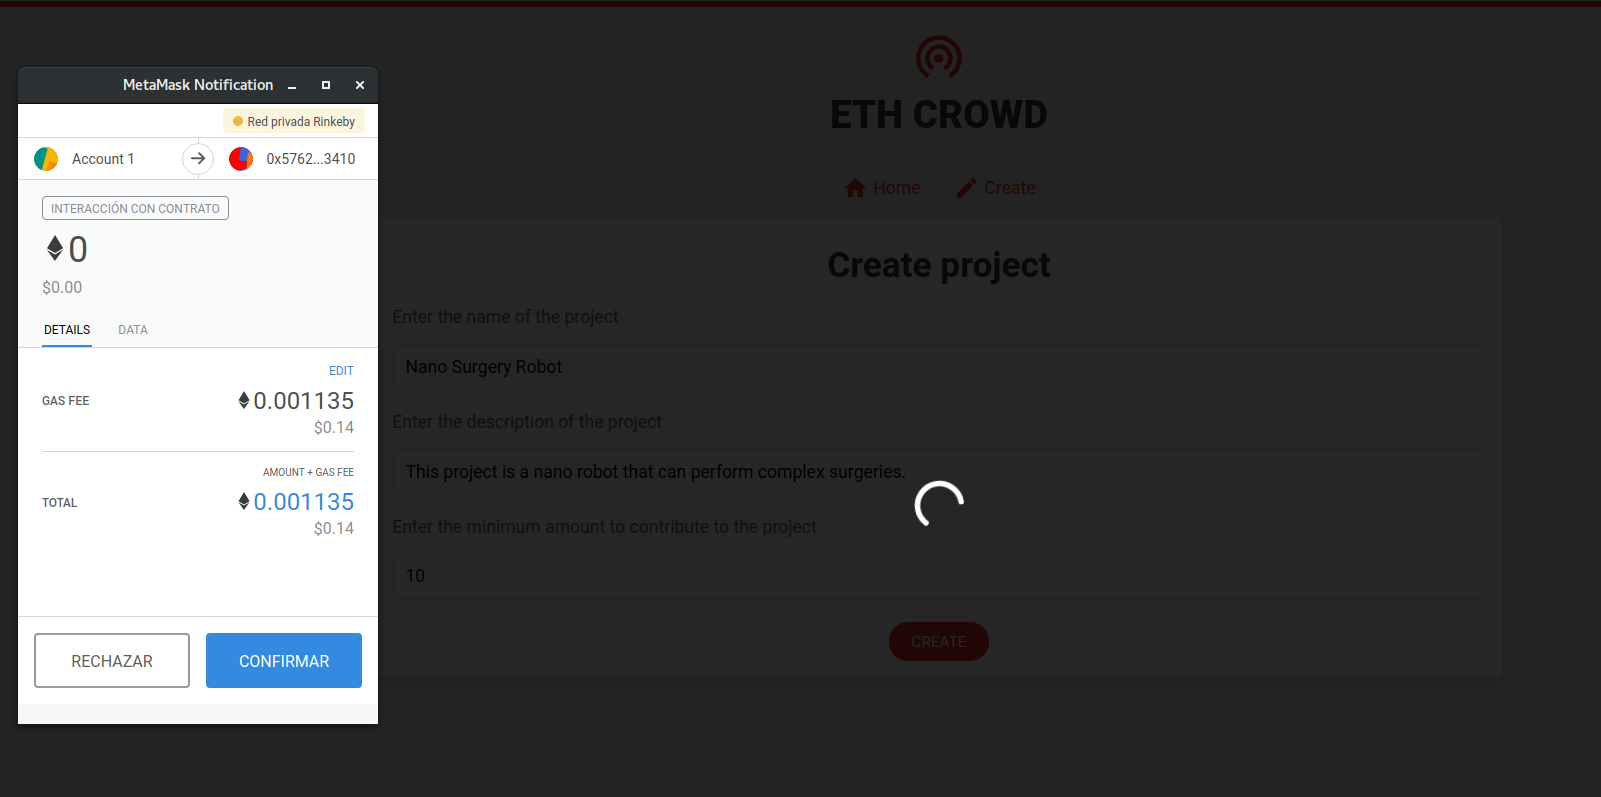
\includegraphics[width=0.9\textwidth]{new-project-metamask}
\caption[new-project-metamask]{En la presente se puede ver cuando Metamask nos pide confirmación para la transacción que está a punto de enviar debido a los costos que ésta tendrá.}
\label{fig:new-project-metamask}
\end{figure}

\begin{figure}[H] 
\centering    
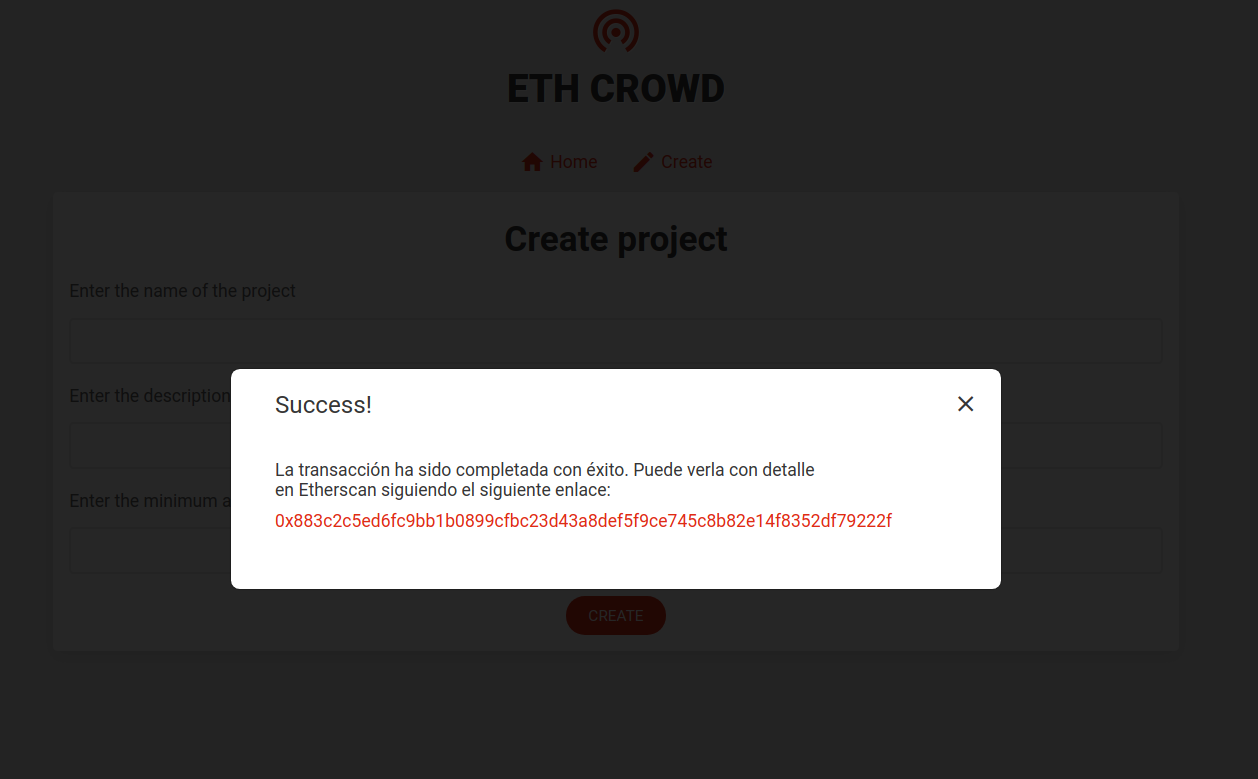
\includegraphics[width=0.9\textwidth]{modal-success}
\caption[modal-success]{Este es el modal utilizado en los casos donde las transacciones se completan con éxito. En el mismo se puede ver el link que dirige a Etherscan, donde se pueden ver detalles de la transacción realizada.}
\label{fig:modal-success}
\end{figure}

\begin{figure}[H] 
\centering    
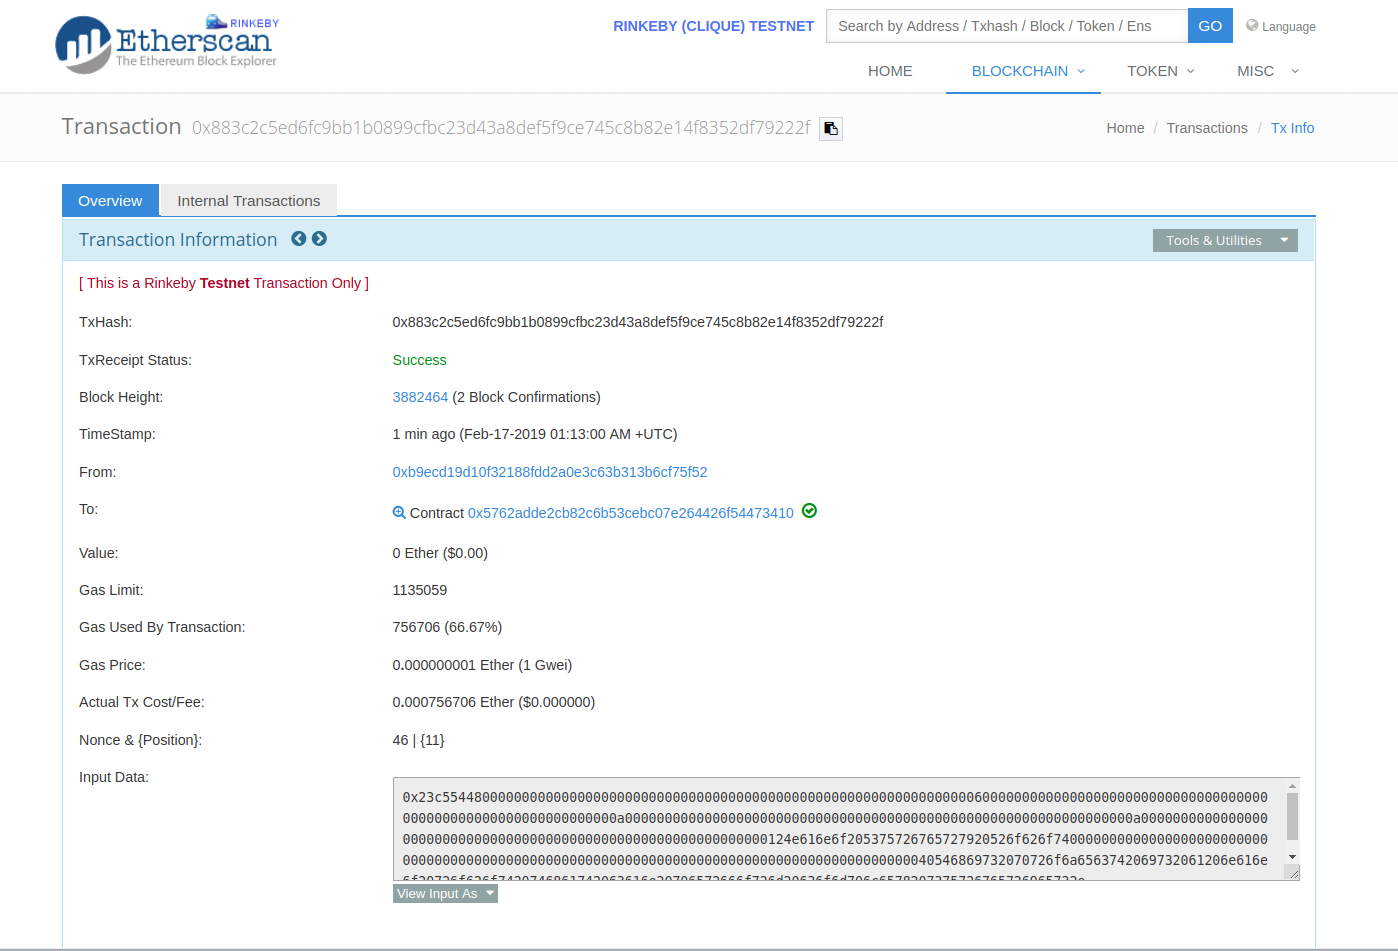
\includegraphics[width=0.9\textwidth]{etherscan-tx}
\caption[etherscan-tx]{Página de Etherscan donde se pueden ver los detalles de la transacción mostrada en la imagen anterior.}
\label{fig:etherscan-tx}
\end{figure}

\begin{figure}[H] 
\centering    
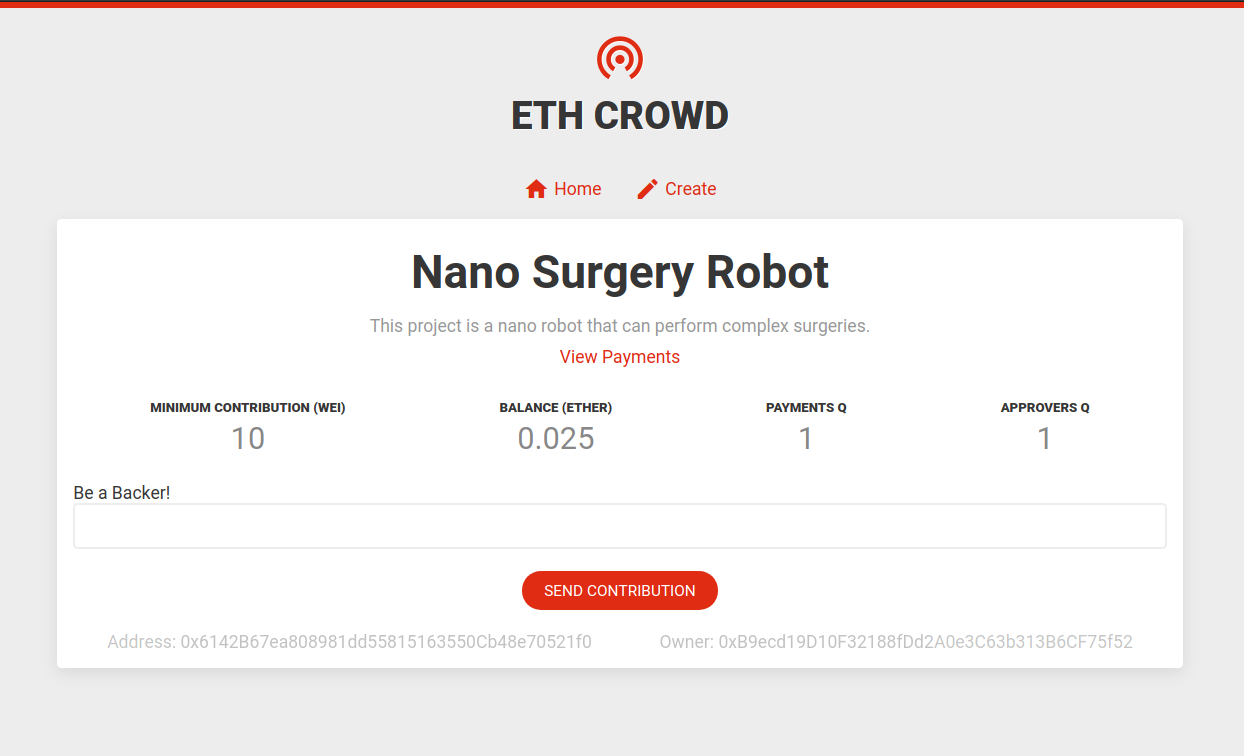
\includegraphics[width=0.8\textwidth]{project-detail}
\caption[project-detail]{Sección de la aplicación donde se puede ver el detalle del proyecto. Este consta del título y descripción del proyecto, un link para ver las solicitudes de pagos del proyecto, la contribución mínima necesaria, el balance de fondos, la cantidad de solicitudes de pago creadas y la cantidad de personas que las aprobaron. Formulario para ser contribuyente, dirección donde está deployado el contrato y dirección del owner del proyecto.}
\label{fig:project-detail}
\end{figure}

\begin{figure}[H] 
\centering    
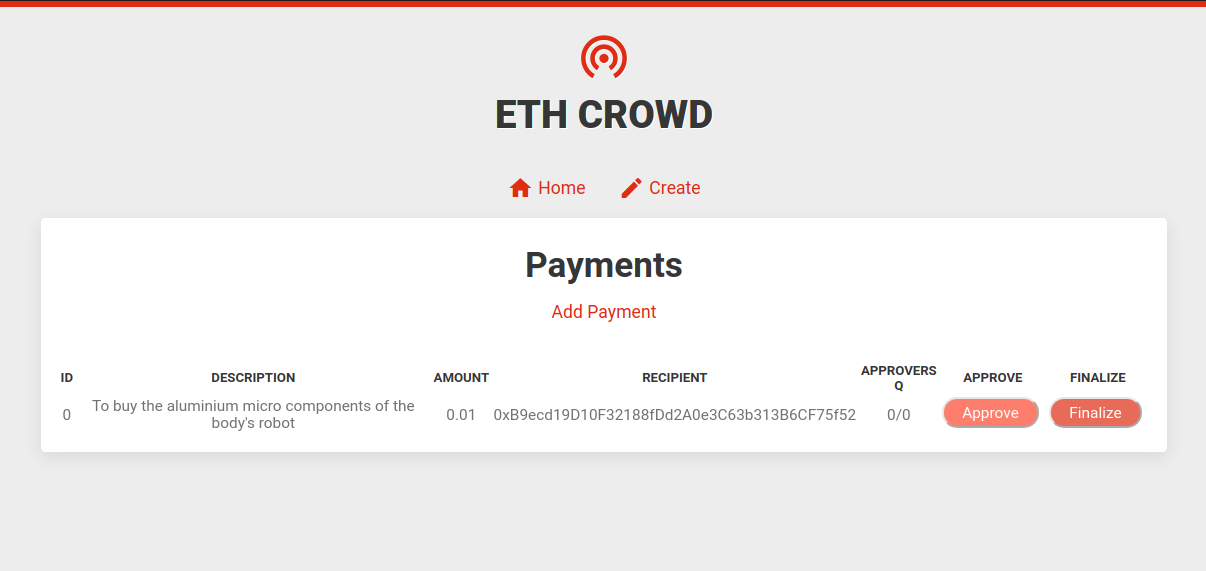
\includegraphics[width=0.9\textwidth]{payments}
\caption[payments]{Aquí se pueden ver listadas las solicitudes de pago del proyecto junto con información y los botones para aprobar el pago o finalizarlo (si se es el owner).}
\label{fig:payments}
\end{figure}

\begin{figure}[H] 
\centering    
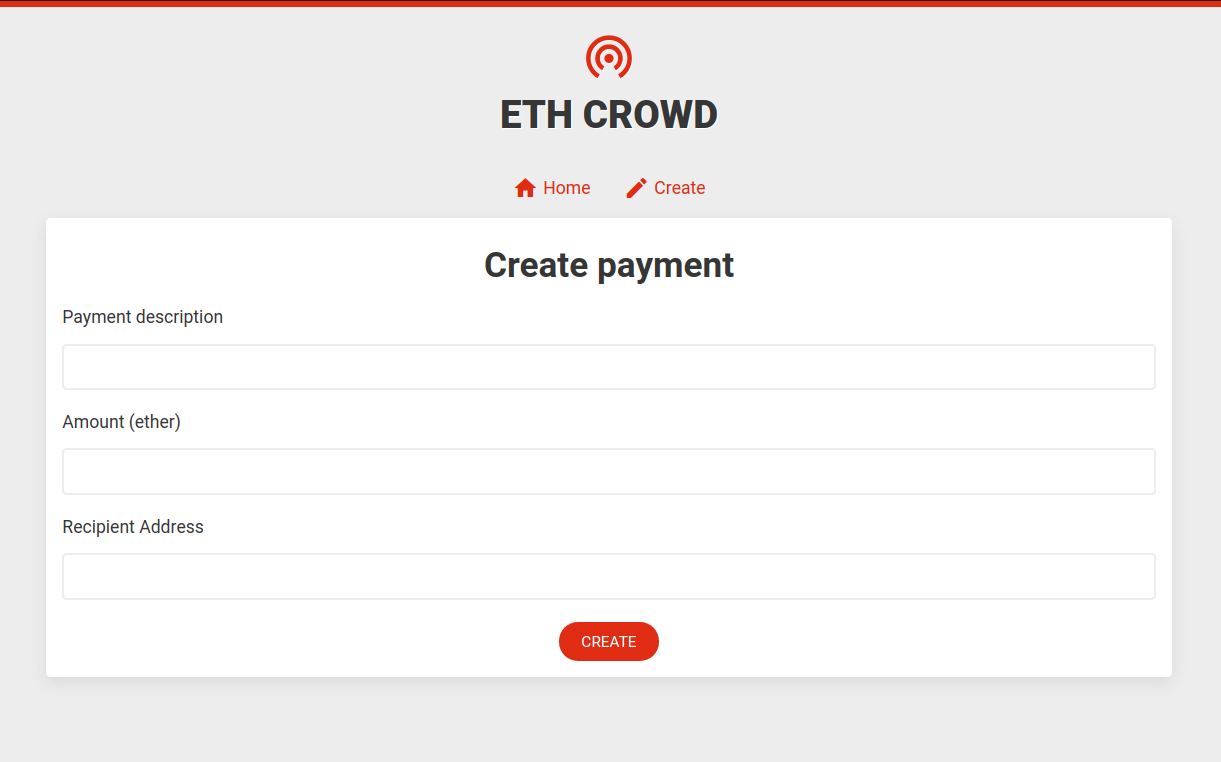
\includegraphics[width=0.9\textwidth]{new-payment}
\caption[new-payment]{Formulario para la creación de una nueva solicitud de pago. Únicamente utilizable por el creador del proyecto.}
\label{fig:new-payment}
\end{figure}


\subsubsection{Scaffolding}

\begin{figure}[H] 
\centering    
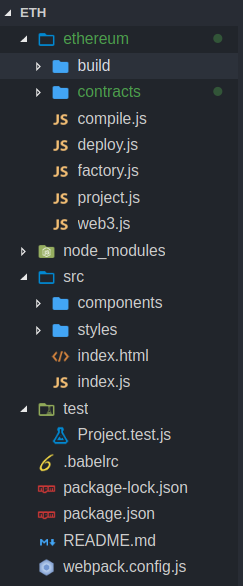
\includegraphics[width=0.4\textwidth]{scaffolding}
\caption[scaffolding]{Scaffolding de la aplicación.}
\label{fig:scaffolding}
\end{figure}


\begin{itemize}
		
	\item ethereum: Dentro de esta carpeta se encuentran los archivos directamente relacionados con 
	el contrato Solidity.
	\begin{itemize}
		\item build: Esta carpeta contiene los archivos compilados resultantes en formato JSON.
			\begin{itemize}
				\item Project.json
				\item ProjectFactory.json
			\end{itemize}
		\item contracts: Dentro se encuentra el contrato Solidity llamado Project.sol
			\begin{itemize}
				\item Project.sol
			\end{itemize}
		\item compile.js: Script para compilar el contrato Project.sol
		\item deploy.js: Script para deployar el contrato Project.sol
		\item factory.js: Script que nos devuelve una instancia de la factory deployada en la dirección que le indiquemos
		\item project.js: Script que nos devuelve una instancia del proyecto en la dirección que le indiquemos
		\item web3.js: Script que detecta si estamos desde el browser o desde node y nos conecta con el contrato en Ethereum
	\end{itemize}
	
	\item node\_modules: Aquí se descargan los paquetes utilizados en los proyectos. Los paquetes se
	encuentran listados en el archivo \textit{package.json}.
	\item src: Aquí dentro se encuentra todo lo relacionado al frontend de la aplicación.
		\begin{itemize}
			\item components: Dentro viven los archivos de los componentes de React creados.
				\begin{itemize}
					\item App.js
					\item Detail.js
					\item Home.js
					\item Modal.js
					\item NewPayment.js
					\item NewProject.js
					\item Payments
				\end{itemize}
			\item styles: Dentro están los archivos de estilos creados.
				\begin{itemize}
					\item app.css
					\item reset.css
				\end{itemize}
			\item index.html
			\item index.js
		\end{itemize}
	
	\item test: Dentro se encuentra el archivo de test del contrato Project.sol
		\begin{itemize}
			\item Project.test.js
		\end{itemize}
	
	\item .babelrc: Archivo de configuración de Babel.
	\item package-lock.json: Archivo autogenerado luego de instalar las dependencias con el comando
	\textit{npm install}.
	\item package.json: Archivo donde tenemos además de información del proyecto, los paquetes utilizados en el mismo
	\item webpack.config.js: Archivo de configuración de webpack.
\end{itemize}

\subsection{Implementación}
En principio se intentó utilizar las últimas versiones LTS disponibles de las tecnologías
seleccionadas para llevar adelante el proyecto pero debido a inconsistencias e incompatibilidades
entre versiones de Node, librerías y solidity se tuvo que trabajar en encontrar un conjunto de
versiones que hagan un ecosistema estable para el desarrollo. Por otra parte, se pudo trabajar con
las últimas versiones estables de React y su ecosistema sin problemas.

Se trabajó con el controlador de versiones Git y la plataforma GitHub para almacenar el
repositorio.

\subsection{Pruebas}
Las pruebas realizadas sobre la aplicación constan por un lado de las pruebas manuales que
cualquier usuario podría hacer en el uso del día a día. Y por otro lado se escribieron tests con
Mocha en la plataforma de Node.js que constaten que la compilación, deploy y métodos del contrato
solidity funcionen correctamente.

Se pospuso para versiones avanzadas el testeo vía código de los componentes React debido a que la
mayoría de ellos depende de conexiones con Ethereum y el contrato para recibir los datos y poder
renderizarse correctamente. Esta tarea es lo que dificulta un poco su testeo total. Una vía de escape
para este problema, es mockear las llamadas a Ethereum y usar dummy data para trabajar durante los
tests automatizados.

\subsection{Versionado}
Como se dijo en la sección de \textit{implementación}, se utilizó Git como sistema de versionado.
Para llevar un control ordenado del código de una manera lo más similar posible a proyectos reales
y de cualquier envergadura (ya sea tanto proyectos pequeños como corporativos a gran escala) se
decidió utilizar parcialmente git flow. 

De manera resumida, git flow propone el uso de ciertas ramas con reglas características de cada
una. Para el desarrollo de la aplicación se usaron las ramas \textit{master, develop} y 
\textit{feature}.

\begin{itemize}
	\item Master
	
	Cualquier commit que se encuentre en esta rama debe estar preparado para subir a producción.
	
	\item Develop
	
	Rama en la que está el código que conformará la siguiente versión planificada del proyecto.
	
	\item Feature
	
	Estas ramas se utilizan para desarrollar nuevas características de la aplicación que, una vez
	terminadas, se incorporan a la rama develop.
	
	Características:
	\begin{itemize}
		\item Se originan a partir de la rama develop.
		\item Se incorporan siempre a la rama develop.
		\item Nombre: cualquiera que no sea master, develop, hotfix-* o release-*
		\begin{wrapfigure}{l}{1\textwidth}
		\centering    
		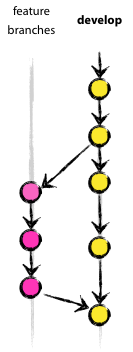
\includegraphics[height=0.3\textheight]{feature_branches}
		\caption[featurebranches]{Diagrama de cómo quedan conformados los commits.}
		\label{fig:feature-branches}
		\end{wrapfigure}
	\end{itemize}

\end{itemize}
